\chapter{Introduction}\label{chp:intro}
%\vspace{-1.5cm}
%\noindent\rule{\columnwidth}{1.2mm}
%\vspace{0.1cm}

The robot development in the last century was able to revolutionize the industry by providing reliability and quality to the production line, since robots often can perform tasks faster, more accurately and with less errors than humans. Human labor that were often repetitive and risky was steadily replaced by robotic labor, with precise movements and increasing automation over time, as shown on \prettyref{fig:robots-per-workers}.

\begin{figure}[!ht]
    \centering
    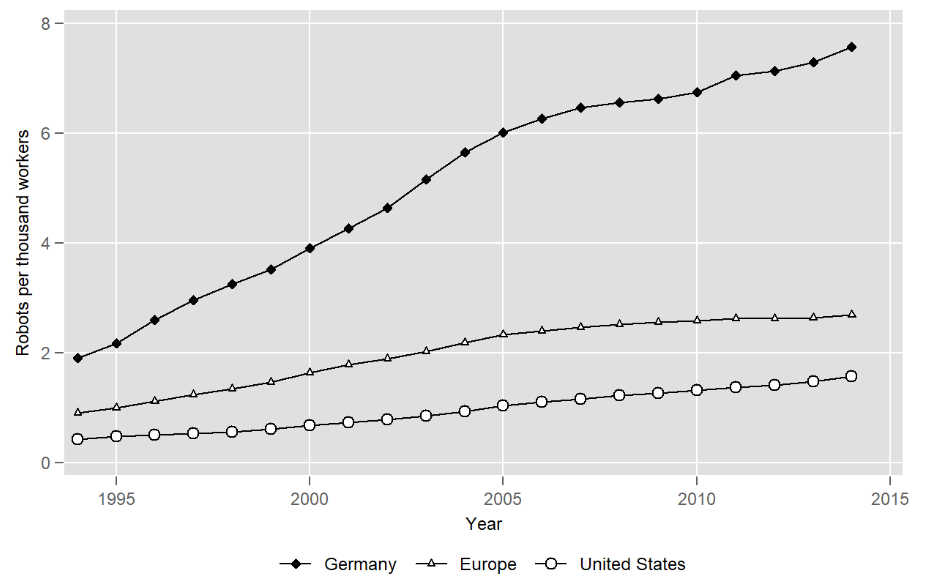
\includegraphics[width=.8\linewidth]{robots-per-workers}
    \caption{Robots per thousand workers in the industry from 1995 to 2014 \cite{dauth2017german}.}
    \label{fig:robots-per-workers}
\end{figure}

Even though robots are increasing present in the industry, using robots to assist persons in every day life might be more challenging. Many authors propose the use of this type of Assistive Robots in places like schools, hospitals and homes, including wheelchair robots, companion robots, manipulator arms for the psychically disabled and elderly populations, etc \cite{feil2005defining}. However, the dynamic and heterogeneous environment, the energy constraints and the safety issues are still issues in domestic use robotics.

According to Feil \cite{feil2005defining}, assistive robots are defined as ones that give support to a human user, whereas socially interactive robots are the ones that merely can interact with humans in the form of gestures, speech, etc. The intersection between this two groups are called socially assistive robots, not focusing on interaction itself but using it as a mechanism to provide aid or assistance.

Fong \cite{fong2003survey} defines 8 traits in socially interactive robots:

\begin{itemize}
    \item Embodiment: defined as the body capabilities of the robot, the morphology an design to deal with the ambient. Social robots design is often taken into consideration because the user must be comfortable engaging with the robot. Also, the amount of sensors and actuators the robot has will expand its capabilities.
    \item Emotion: complements the embodiment in the robots by interacting in a social context. Integrating emotion in robots can create empathy and make people threat the them like they threat other humans. Emotions can be displayed both as expression, in the form of moving lips, eyebrows, eyes and LEDs, as well as in the form of speech, in voice tone, loudness and pitch. Body language also takes place in full-body robots.
    \item Dialogue: Creating meaningful dialogue between two or more parties is hard in the form of low-level dialogue and natural language are still features under development and remain a great challenge to robots. Robots can also use dialog in a non-verbal way, communicating in gestures and facial display, in addition to displaying emotions.
    \item Personality: in order to correlate with users, robots must develop personality traits that will 
    \item Human-oriented perception: to interact, robots must perceive the environment as humans do. In social situations, this includes people tracking, speech recognition, gesture recognition and facial perception.
    \item User modeling: in addition to design and perception, the must act based on people personality, learning the user's personality to create a model on how to react.
    \item Socially situated learning: continuously learning for improving communication or acquiring new skills is essential, whether by teaching or imitation.
    \item Intentionality: lastly, humans must feel that the robot has a purpose and acts rationally. This can be achieved by demonstrating goal-directed behaviors or demonstrating attention to key objects in the scenario.
\end{itemize}

Feil goes further and defines socially assistive robot with additional properties relative to Fong's definition:

\begin{itemize}
    \item User Populations: defines the characteristics of the user, like age, impairment and need. He categorizes the user populations as Elderly, Individuals with Physical Impairments, Individuals in Convalescent Care, Individuals With Cognitive Disorders and Students.
    \item Task: the author cites as task examples Tutoring, Physical Therapy, Daily Life Assistance and Emotional Expression. 
    \item Sophistication of Interaction: the robot must develop beyond the emotional feature described by Fong, evolving into more complex reciprocal interactions with the user.
    \item Role of the Assistive Robot: the role of the assistive robot must reflect into it's appearance and behaviour, affecting both embodiment and personality, depending on the task and nature of interaction.
\end{itemize}

\begin{figure}[!ht]
    \centering
    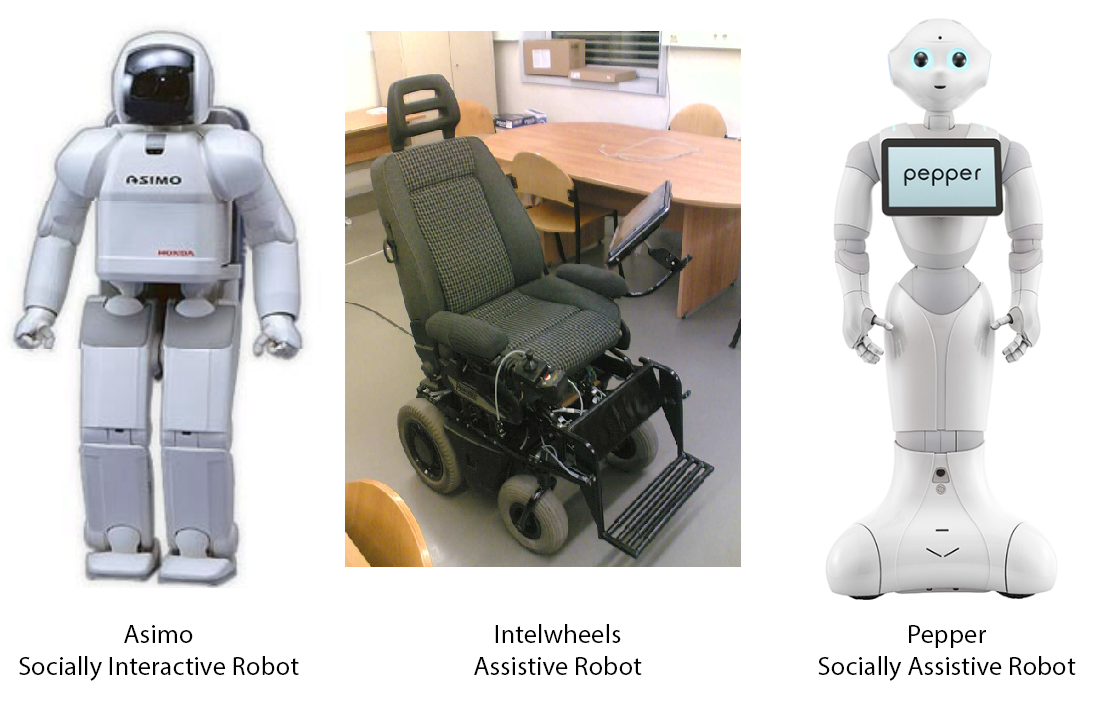
\includegraphics[width=\linewidth]{social-assistive-robots}
    \caption{Examples of Assistive and Social robots \cite{sakagami2002intelligent,braga2008intellwheels,tanaka2015pepper}.}
    \label{fig:social-assistive-robots}
\end{figure}

One of the most famous socially interactive robot developed is ASIMO, a human-like robot developed by the Japanese company Honda in 2000. It featured a pair of legs and many features and sensors that would later be integrated into other assistive robots. Its main task was to meet visitors in the meeting room and to guide them once the manager confirms their identity. It was able to perform navigation and obstacle avoidance, respond to voice and gesture calls \cite{sakagami2002intelligent}. Even though the can interact with people, it does not qualify as a socially assistive robot (the first version, at the time) as defined by Feil because it couldn't fit in the user populations described. The robot as later improved to have greater grasping capabilities and a more robust sensor set.

Intelwheels is an example of a assistive robot. It can assist handicapped people operating an electric wheelchair, providing not only user operation with collision avoidance but autonomous navigation. It can help elders and people with physical impairments, but the user input is one-way: it can recognize voice and facial expressions but won't interact back with the user \cite{braga2008intellwheels}.

The Pepper, developed to fit into the category of both Emotional Expression and Tutoring. It was aimed at the concept of the robot learning together with children using a the robot display to teach English, characterizing it as a socially assistive robot. A remote human teacher would help the process by orienting the classes. Instead of just showing the contents in the screen creating boredom, the robot engaged in playful activities with the kids, including telling them to search for a specific object in the room or repeating gestures with the robot, compelling the children to participate actively \cite{tanaka2015pepper}.

The Care-o-bot, or COB, for short, is described as a robotic home assistant aimed at helping people with mobility impairments in their daily life. The target group include elders, disabled persons, with health conditions and with movement restraints. His tasks include setting the table, carrying objects like books and drinks around, dealing with medication, helping the patients standing up, as well as serving as a companion to the person. The robot can also do other tasks usually performed by a nurse or doctor, like monitoring the patient with conditions in their daily routines, reminding them to take medication and calling emergency in case of an incident \cite{graf2004care}.

\begin{figure}[!ht]
    \centering
    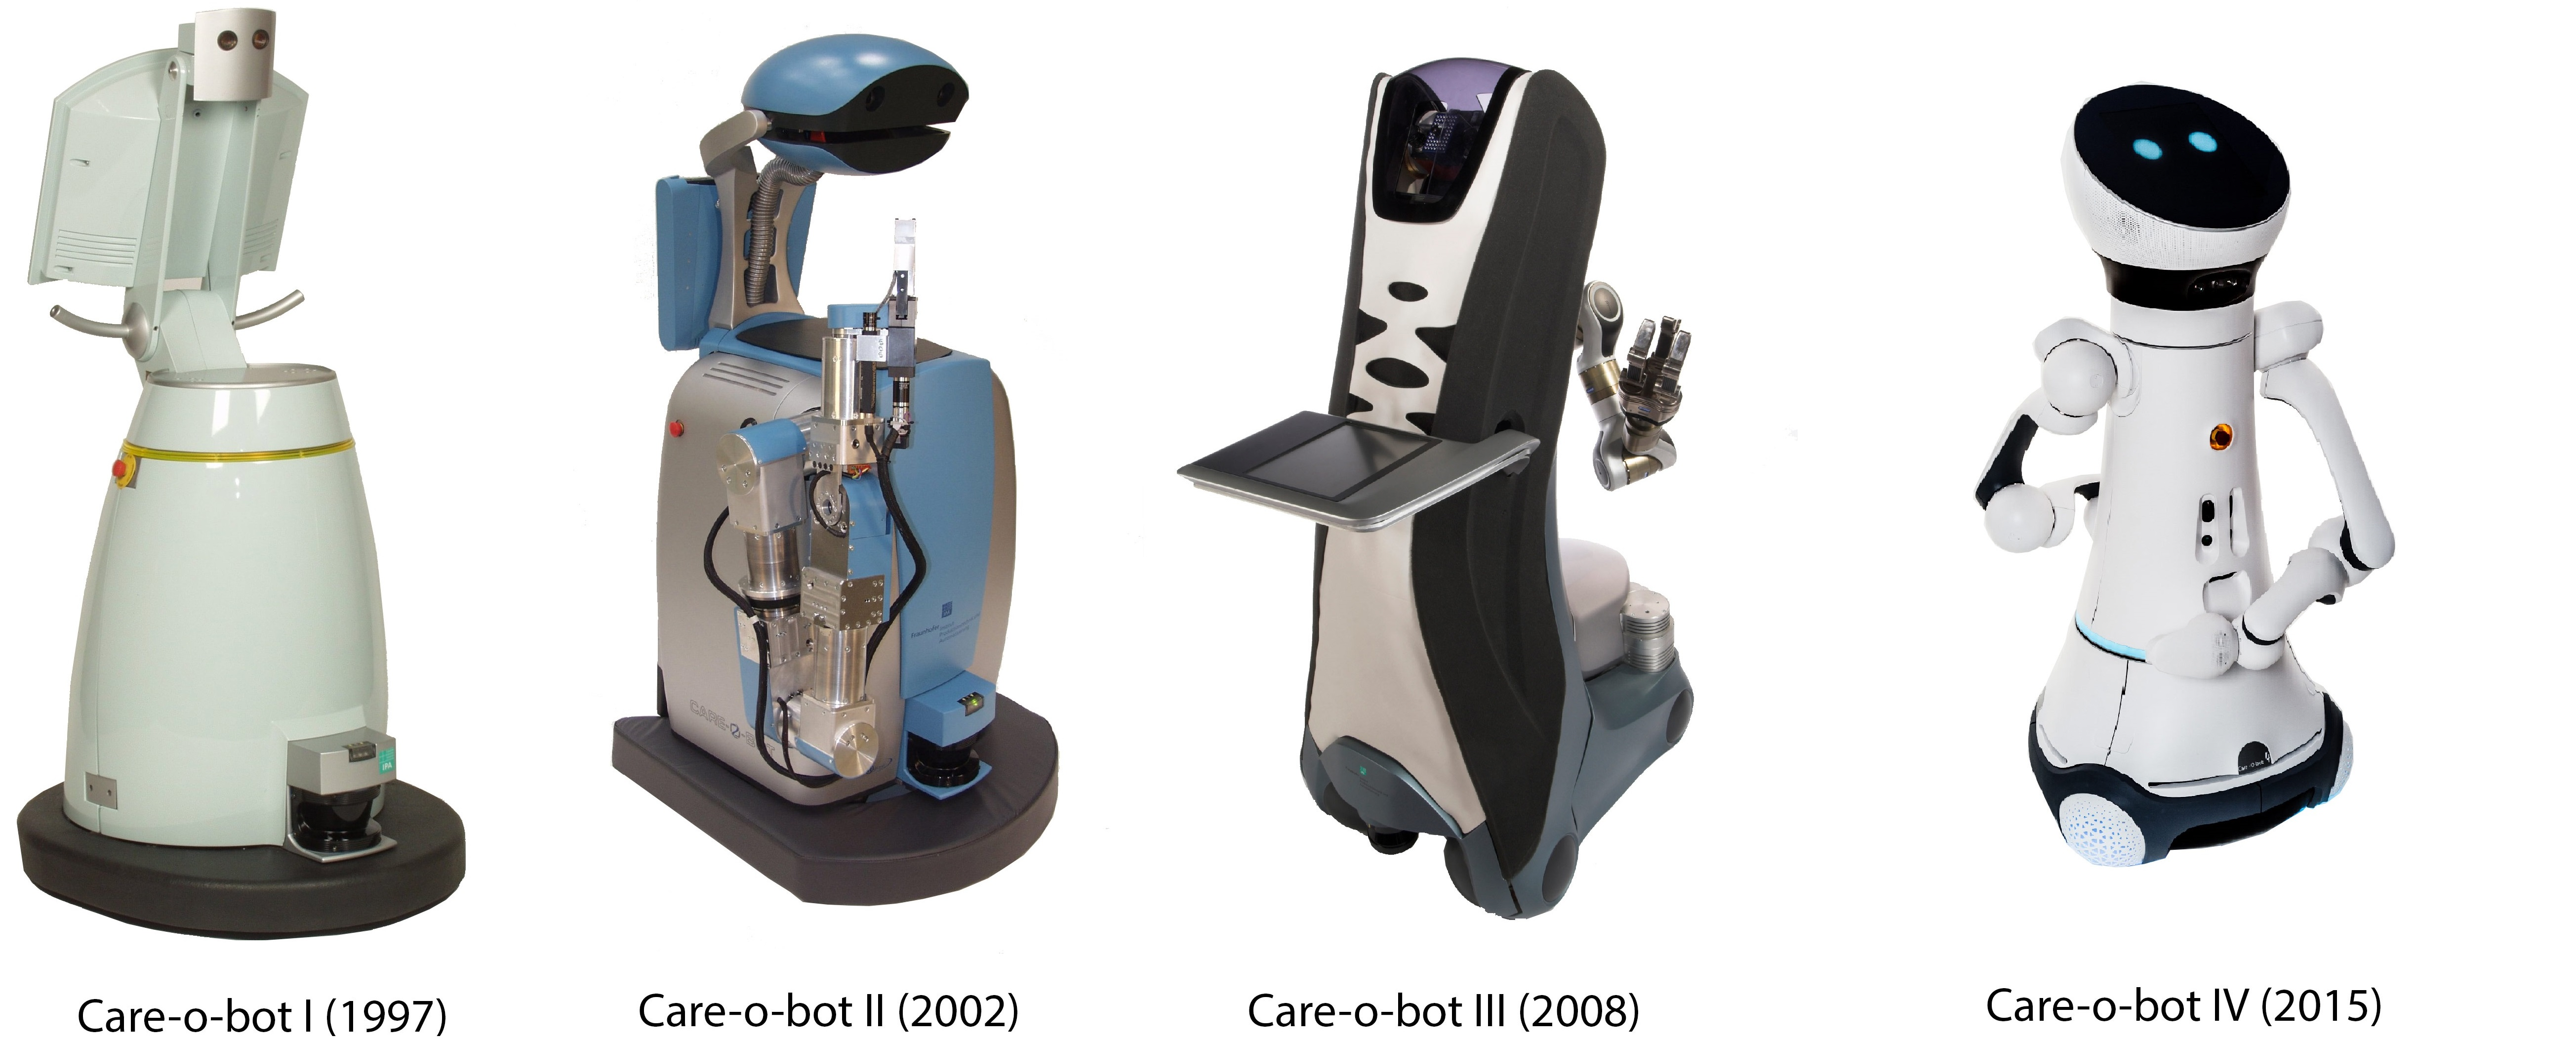
\includegraphics[width=\linewidth]{cob-evo}
    \caption{Evolution of Care-o-bot.}
    \label{fig:cob-evo}
\end{figure}

The Care-o-bot evolution throughout the years can be seen on \prettyref{fig:cob-evo}. The first prototype was built in 1997, but lacked many features and was a relatively new idea. It was soon followed by Care-o-bot II, in 2002, equipped with a manipulator, two cameras, laser scanners and a hand held control panel. The version II presented great improvements in navigation, computer vision and manipulation, but was still rudimentary, having problems in low light conditions and dynamic environments (the 3D scans could only be run once because of processing constraints) and not being recommended inexperienced users \cite{graf2004care}.

The third generation came in 2008, using a better 7DOF arm and 3 finger gripper with tactile feedback. It also became a lot more user friendly, applying the concepts of embodiment and presenting a less bulkier body with smoother surfaces and less visible mechanical parts. The robot body was divided into a working side (in the back, where the manipulator stands) and a serving side (on the front, to interact with users) \cite{graf2009robotic}.

The fourth generation, presented in 2015, and focused heavily on emotion design. It was developed to appear familiar and sociable, and avoid the uncanny valley, where human-like robots can cause strangeness or even fear. It featured a multi-modal user interface capable of displaying facial expressions with a minimalistic pair of eyes to display a wide range of emotions. The spherical joints in the torso and head allow more agility, the body is smaller and more efficient and more sensors and 3D cameras were installed.


%state the general topic and give some background

%provide a review of the literature related to the topic

%define the terms and scope of the topic

%outline the current situation

%evaluate the current situation (advantages/ disadvantages) and identify the gap

%identify the importance of the proposed research

%state the research problem/ questions

%state the research aims and/or research objectives

%state the hypotheses

%outline the order of information in the thesis

%outline the methodology